\documentclass[11pt,a4paper]{article}
\usepackage[margin=2.5cm]{geometry}
\usepackage[T1]{fontenc}
\usepackage{amsmath,amssymb,amsthm,mathtools,bm}
\usepackage{tcolorbox}
\usepackage{enumitem}
\usepackage{tikz}
\usepackage[colorlinks=true,linkcolor=blue!50!black,citecolor=blue!50!black]{hyperref}
\setlength{\parindent}{0pt}\setlength{\parskip}{6pt}
\numberwithin{equation}{section}
\linespread{1.08}

\newtcolorbox{dove}{colback=gray!6,colframe=gray!60!black,title=Dove siamo e perché,fonttitle=\bfseries}
\newtcolorbox{idea}{colback=blue!4,colframe=blue!45!black,title=L'idea in parole,fonttitle=\bfseries}
\newtcolorbox{porta}{colback=green!4,colframe=green!40!black,title=Cosa portiamo via,fonttitle=\bfseries}
\newtcolorbox{attento}{colback=red!4,colframe=red!50!black,title=Attenzione,fonttitle=\bfseries}
\newtheorem{prop}{Proposizione}
\theoremstyle{remark}
\newtheorem*{oss}{Osservazione}

\newcommand{\Tr}{\mathrm{Tr}}
\newcommand{\Hf}{\mathcal{H}}
\newcommand{\G}{\mathcal{G}}
\newcommand{\Hg}{\mathcal{H}_0}
\newcommand{\p}{\mathfrak{p}}
\newcommand{\h}{\mathfrak{h}}
\newcommand{\one}{\mathbb{1}}
\newcommand{\R}{\mathbb{R}}

\title{\textbf{Guida ragionata al paper}\\[4pt]\Large Higgs radial modes in linear completions of non-linear sigma models\\[6pt]
\normalsize Seguendo il filo logico: che cosa si fa, perché, e come si fa}
\author{Note per Giulio Marino}
\date{Novembre 2026}

\begin{document}
\maketitle

\begin{abstract}
Queste note accompagnano la lettura del paper un passo alla volta. Ogni capitolo comincia dicendo \emph{a che punto della storia siamo} e \emph{perché} ci serve quello che stiamo per fare. Poi dà l'idea in parole e solo dopo fa il conto, commentando ogni passaggio. Alla fine riassume cosa ci portiamo dietro. Si parte da un esempio che si fa tutto a mano, il modello $O(N)$, cioè la versione ``giocattolo'' dell'Higgs del Modello Standard, e da lì si costruisce tutto il resto. Le note precedenti (\texttt{notes.pdf}) restano utili come formulario con i conti compatti; queste invece spiegano.
\end{abstract}

\tableofcontents
\newpage

%=====================================================================
\section{Come leggere queste note}
%=====================================================================

Il paper risponde a \emph{una} domanda:
\begin{center}
\fbox{\parbox{0.85\textwidth}{\centering\emph{Se una teoria di bosoni di Goldstone smette di funzionare ad alte energie, quali particelle nuove (``modi radiali'') bisogna aggiungere per aggiustarla, e quante ne servono davvero?}}}
\end{center}
Tutto il resto è al servizio di questa domanda. La catena logica è:

\begin{enumerate}[label=\textbf{\arabic*.}]
\item I Goldstone interagiscono con derivate, quindi le loro ampiezze crescono con l'energia: la teoria non può valere sempre (Cap.~\ref{cap:problema}).
\item Nel caso più semplice (Higgs del Modello Standard) si vede esplicitamente come un modo radiale, l'Higgs, cancella la crescita (Cap.~\ref{cap:toy}).
\item Si capisce la ragione geometrica: la crescita misura la \emph{curvatura} dello spazio dei vuoti, e i modi radiali misurano quanto questo spazio è \emph{piegato} dentro uno spazio più grande e piatto. La relazione tra le due cose è l'equazione di Gauss (Capp.~\ref{cap:geo}--\ref{cap:gauss}).
\item Dall'equazione di Gauss si deducono risultati generali, validi per qualunque completamento (Cap.~\ref{cap:gauss}).
\item Per i tre coset del paper si costruisce il completamento ``naturale'' e lo si scrive in modo compatto (Capp.~\ref{cap:gruppi}--\ref{cap:lineare}).
\item Si dimostra che funziona per i tre coset insieme, grazie a un'identità tra commutatori e anticommutatori (Cap.~\ref{cap:cuore}).
\item Si stabilisce quali modi radiali sono indispensabili (Capp.~\ref{cap:quali}--\ref{cap:rigid}).
\item Si stimano le masse dei modi radiali (unitarietà) e si guardano le conseguenze fisiche (Capp.~\ref{cap:unit}--\ref{cap:e6}).
\end{enumerate}

\textbf{Corrispondenza con il paper} (versione da 23 pagine):
\begin{center}
\begin{tabular}{ll}
\hline
Sezione del paper & Capitoli di queste note\\
\hline
I. Introduzione & \ref{cap:problema}, \ref{cap:toy}, \ref{cap:domanda}\\
II. Symmetric cosets and linear completions & \ref{cap:geo}, \ref{cap:gauss}, \ref{cap:ccwz}\\
III. Group theory: matrix representations & \ref{cap:gruppi}\\
IV. Linear sigma model in polar coordinates & \ref{cap:lineare}\\
V. NGB scattering and necessity & \ref{cap:cuore}, \ref{cap:quali}\\
VI. Beyond the minimal representation & \ref{cap:rigid}\\
VII. Perturbative unitarity & \ref{cap:unit}\\
VIII--IX. Electroweak, charged radials & \ref{cap:ew}\\
X. Running & \ref{cap:unit}\\
Nuove sezioni (LEC, $N=4$, QCD, $E_6/F_4$) & \ref{cap:rigid}, \ref{cap:unit}, \ref{cap:lec}, \ref{cap:e6}\\
\hline
\end{tabular}
\end{center}

\textbf{Convenzioni minime.}
\begin{itemize}[nosep]
\item Metrica $(+,-,-,-)$. Per lo scattering $1+2\to3+4$: $s=(p_1+p_2)^2$, $t=(p_1-p_3)^2$, $u=(p_1-p_4)^2$. Per particelle senza massa $s+t+u=0$.
\item ``Ampiezza'' $\mathcal A$: è il numero il cui modulo quadro dà la probabilità. Si calcola con i diagrammi di Feynman: $i\mathcal A=$ somma dei diagrammi.
\end{itemize}

%=====================================================================
\section{Il problema fisico: perché i Goldstone ``rompono'' la teoria}
\label{cap:problema}
%=====================================================================

\begin{dove}
Siamo all'inizio dell'introduzione del paper. Prima di qualunque formula bisogna capire \emph{che cosa non funziona} nei modelli sigma non lineari: è il motivo per cui il paper esiste.
\end{dove}

\subsection{Rottura spontanea e bosoni di Goldstone}

Una teoria ha una simmetria globale $\G$, ma il vuoto (lo stato di minima energia) è invariante solo sotto un sottogruppo $\Hg$. Questa è la rottura spontanea. Il teorema di Goldstone dice che per ogni direzione di simmetria rotta esiste una particella senza massa, il bosone di Goldstone (NGB). Il numero di NGB è $\dim\G-\dim\Hg$.

\textbf{Immagine utile.} Pensa al potenziale a ``cappello messicano''. I vuoti formano un cerchio (o una sfera, o in generale una varietà): sono tutti equivalenti per simmetria. Muoversi \emph{lungo} il fondo del cappello non costa energia, e queste sono le eccitazioni senza massa, i Goldstone. Muoversi \emph{verso l'alto}, lontano dal fondo, costa energia, e queste sono le eccitazioni massive, i \textbf{modi radiali}. L'Higgs del Modello Standard è esattamente il modo radiale del cappello messicano elettrodebole.

L'insieme dei vuoti è il \textbf{coset} $\G/\Hg$. I campi dei Goldstone $\pi^a(x)$ sono coordinate su questo spazio.

\subsection{Il modello sigma non lineare}

Se ci interessano solo le energie molto più basse della massa dei modi radiali, possiamo ``congelare'' questi ultimi e tenere solo i Goldstone. Il risultato è il modello sigma non lineare (NL$\Sigma$M): una teoria con soli NGB, vincolati a vivere sul coset. La Lagrangiana più generale con due derivate è
\begin{equation}
\mathcal L=\tfrac12\,g_{ab}(\pi)\,\partial_\mu\pi^a\partial^\mu\pi^b ,
\end{equation}
dove $g_{ab}(\pi)$ è la \emph{metrica} del coset, cioè il modo in cui si misurano le distanze sulla varietà dei vuoti. La costante $f$ (costante di decadimento) fissa la ``taglia'' del coset: è il raggio del cappello messicano.

\textbf{Perché le interazioni hanno derivate.} Un NGB a impulso nullo corrisponde a una rotazione globale del vuoto, che non cambia la fisica. Quindi a impulso zero i Goldstone non interagiscono. Le interazioni devono sparire quando $p\to0$, e questo è possibile solo se contengono derivate.

\subsection{Perché le ampiezze crescono}

Un'interazione con due derivate, per esempio $\frac{1}{f^2}\pi\pi\,\partial\pi\partial\pi$, dà un'ampiezza proporzionale a due impulsi:
\[
\mathcal A(\pi\pi\to\pi\pi)\sim\frac{p^2}{f^2}\sim\frac{s}{f^2}.
\]
Più è alta l'energia, più grande è l'ampiezza. Ma un'ampiezza non può crescere senza limite: la probabilità non può superare 1. Questo vincolo si chiama \textbf{unitarietà}. In pratica si scompone l'ampiezza in onde parziali $a_\ell$ e si richiede $|{\rm Re}\,a_\ell|\le\frac12$. Con $a_0\sim s/(16\pi f^2)$ il vincolo è violato per $\sqrt s\gtrsim$ qualche $f$. Si dice che a quella scala ``si perde l'unitarietà perturbativa'': la teoria diventa fortemente accoppiata, oppure deve entrare fisica nuova.

\subsection{Le due vie d'uscita}

\begin{itemize}
\item \textbf{Accoppiamento forte.} È quello che succede in QCD: i pioni sono i Goldstone della simmetria chirale, e sopra $\sim1$ GeV entra la dinamica forte dei quark (risonanze larghe, $\rho$, $f_0(500)$, \ldots).
\item \textbf{Completamento debole.} Si aggiungono nuove particelle debolmente accoppiate, i modi radiali, che cancellano la crescita. La teoria che le contiene è il \textbf{modello sigma lineare} (L$\Sigma$M). È ciò che fa il Modello Standard con l'Higgs.
\end{itemize}
Il paper studia la seconda via.

\subsection{Il caso che tutti conoscono: $W_LW_L$ e l'Higgs}

Nel Modello Standard i tre Goldstone della rottura elettrodebole vengono ``mangiati'' e diventano le polarizzazioni longitudinali di $W^\pm$ e $Z$. Il teorema di equivalenza dice che ad alte energie $\mathcal A(W_LW_L\to W_LW_L)\simeq\mathcal A(\pi\pi\to\pi\pi)$. Senza Higgs questa ampiezza cresce come $s/v^2$ ($v=246$ GeV) e l'unitarietà è persa intorno a 1 TeV. Era il ``no-lose theorem'' di LHC: o si trova l'Higgs, o si vede una dinamica forte. Con l'Higgs la crescita si cancella esattamente. Nel prossimo capitolo lo verifichiamo a mano.

\begin{porta}
\begin{itemize}[nosep]
\item I Goldstone interagiscono con derivate, quindi $\mathcal A\sim s/f^2$ cresce.
\item La crescita viola l'unitarietà a energie di qualche $f$.
\item Un completamento debole aggiunge modi radiali che cancellano la crescita.
\item La domanda del paper: per coset più complicati della sfera, quali modi radiali servono?
\end{itemize}
\end{porta}

%=====================================================================
\section{L'esempio giocattolo: il modello $O(N+1)$, fatto tutto a mano}
\label{cap:toy}
%=====================================================================

\begin{dove}
Prima di affrontare i coset complicati, facciamo per intero il caso più semplice, in cui tutto si calcola in mezza pagina. Tutte le strutture del paper compaiono già qui: due sistemi di coordinate, la cancellazione tra contatto e scambio, il legame tra accoppiamento e curvatura. Quando nel paper ti perdi, torna a questo capitolo.
\end{dove}

\subsection{Il modello}

Prendi $N+1$ campi scalari reali $\phi=(\phi_1,\dots,\phi_{N+1})$ con
\begin{equation}
\mathcal L=\tfrac12(\partial\phi)^2-\frac{\lambda}{4}\big(\phi^2-v^2\big)^2 .
\end{equation}
Sono simmetrici sotto rotazioni $O(N+1)$. Il minimo è a $|\phi|=v$: i vuoti formano una sfera $S^N$ di raggio $v$. Scegliamo il vuoto $\phi=(0,\dots,0,v)$, che è invariante solo sotto le rotazioni $O(N)$ che lasciano fisso l'ultimo asse. Si ha quindi $\G=O(N+1)$, $\Hg=O(N)$ e $N$ Goldstone.

Per $N=3$ questo è esattamente il settore di Higgs del Modello Standard: $SO(4)/SO(3)\simeq SU(2)\times SU(2)/SU(2)$, con $v=246$ GeV, tre Goldstone e un Higgs.

\subsection{Primo modo di contare: coordinate cartesiane}

Scriviamo $\phi=(\pi_1,\dots,\pi_N,\ v+\sigma)$, cioè spostiamo semplicemente l'origine nel vuoto. Allora $\phi^2-v^2=\pi^2+2v\sigma+\sigma^2$ e il potenziale diventa
\[
V=\lambda v^2\sigma^2+\lambda v\,\sigma(\sigma^2+\pi^2)+\frac\lambda4(\sigma^2+\pi^2)^2 .
\]
Leggiamo:
\begin{itemize}[nosep]
\item massa del $\sigma$: $m^2=2\lambda v^2$ (i $\pi$ restano senza massa, come previsto);
\item vertice cubico $\sigma\pi\pi$: dal termine $-\lambda v\,\sigma\pi^2$ nella Lagrangiana;
\item vertice quartico $\pi\pi\pi\pi$: dal termine $-\frac\lambda4(\pi^2)^2$.
\end{itemize}
\textbf{Nessuna derivata nelle interazioni.} Questo è il punto chiave delle coordinate cartesiane.

\textbf{Ampiezza $\pi_a\pi_b\to\pi_c\pi_d$.} Per la simmetria $O(N)$ ha la forma
\[
\mathcal A=A(s,t,u)\delta_{ab}\delta_{cd}+A(t,s,u)\delta_{ac}\delta_{bd}+A(u,t,s)\delta_{ad}\delta_{bc}.
\] Basta calcolare la funzione $A(s,t,u)$, il coefficiente di $\delta_{ab}\delta_{cd}$:
\begin{itemize}
\item \emph{Contatto.} Derivando $(\pi^2)^2=\pi_e\pi_e\pi_f\pi_f$ quattro volte si ottiene $8(\delta_{ab}\delta_{cd}+\dots)$. Il vertice è quindi $-i\frac\lambda4\cdot8=-2i\lambda$ per la struttura $\delta_{ab}\delta_{cd}$, e il contributo ad $A$ è $-2\lambda$.
\item \emph{Scambio di $\sigma$ nel canale $s$.} Il vertice è $-i\lambda v\cdot2=-2i\lambda v$ (il fattore 2 viene dai due modi di attaccare i due $\pi$). Due vertici e un propagatore danno $i\mathcal A=(-2i\lambda v)^2\frac{i}{s-m^2}$, cioè un contributo $-\frac{4\lambda^2v^2}{s-m^2}$.
\end{itemize}
Sommando e usando $m^2=2\lambda v^2$:
\begin{equation}
A(s,t,u)=-2\lambda-\frac{4\lambda^2v^2}{s-m^2}=-2\lambda\,\frac{s-m^2+m^2}{s-m^2}=\boxed{-\frac{m^2}{v^2}\,\frac{s}{s-m^2}} .
\label{eq:toyA}
\end{equation}
Guardiamo i due limiti:
\begin{itemize}
\item \textbf{basse energie} ($s\ll m^2$): $A\simeq\frac{m^2}{v^2}\frac{s}{m^2}=\frac{s}{v^2}$. È l'ampiezza dei soli Goldstone, cioè il NL$\Sigma$M (formula di Weinberg per i pioni). Cresce con $s$.
\item \textbf{alte energie} ($s\gg m^2$): $A\to-\frac{m^2}{v^2}=-2\lambda$, una costante. L'ampiezza è \emph{limitata}.
\end{itemize}
In coordinate cartesiane la limitatezza è ovvia: senza derivate, i diagrammi sono costanti o decrescono come $1/s$. La crescita $s/v^2$ a basse energie è il ``residuo'' di una cancellazione tra contatto e scambio, che lasciano un termine $\propto s/m^2$.

\subsection{Secondo modo di contare: coordinate polari}

Ora scriviamo il campo come ``raggio $\times$ direzione'':
\[
\phi=(v+h)\,\vec n(\pi),\qquad |\vec n|=1,\qquad \vec n=\Big(\frac{\pi_1}{v},\dots,\frac{\pi_N}{v},\ \sqrt{1-\pi^2/v^2}\Big).
\]
Qui $h$ misura quanto ci si allontana dalla sfera dei vuoti (il modo radiale) e i $\pi$ dicono dove ci si trova sulla sfera (i Goldstone). È la parametrizzazione ``naturale'' per vedere i Goldstone, perché il potenziale dipende solo da $|\phi|=v+h$ e i $\pi$ non compaiono nel potenziale.

Il termine cinetico:
\[
\tfrac12(\partial\phi)^2=\tfrac12(\partial h)^2+\tfrac12(v+h)^2(\partial\vec n)^2 ,\qquad(\partial\vec n)^2=\frac{(\partial\pi)^2}{v^2}+\frac{(\pi\cdot\partial\pi)^2}{v^2(v^2-\pi^2)} .
\]
\emph{Verifica} dell'ultima formula: $\partial n_{N+1}=-\frac{\pi\cdot\partial\pi}{v^2\sqrt{1-\pi^2/v^2}}$, il cui quadrato dà il secondo termine. Sviluppando:
\begin{equation}
\mathcal L=\tfrac12(\partial\pi)^2+\tfrac12(\partial h)^2+\underbrace{\frac{1}{2v^2}(\pi\cdot\partial\pi)^2}_{\text{contatto NL}\Sigma\text{M}}+\underbrace{\frac1v\,h\,(\partial\pi)^2}_{\text{accoppiamento }h\pi\pi}+\dots
\label{eq:toypolar}
\end{equation}
\textbf{Adesso le interazioni hanno derivate.} Il contatto a quattro $\pi$ è quello del NL$\Sigma$M e l'Higgs si accoppia ai Goldstone con derivate, con forza $1/v$.

\textbf{Ampiezza nelle coordinate polari.}
\begin{itemize}
\item \emph{Contatto} da $\frac{1}{2v^2}(\pi\cdot\partial\pi)^2$. Si calcola come prima: per la struttura $\delta_{ab}\delta_{cd}$ servono le assegnazioni in cui le derivate cadono una su una gamba della coppia $\{1,2\}$ e l'altra su una gamba della coppia $\{3,4\}$. Con momenti tutti entranti, $(p_1+p_2)\cdot(p_3+p_4)=-s$, e il risultato è $A_{\rm contatto}=+\frac{s}{v^2}$. Cresce.
\item \emph{Scambio di $h$.} Il vertice da $\frac1vh(\partial\pi)^2$ è $i\frac1v\cdot2\cdot(-ip_1)\cdot(-ip_2)=-\frac{2i}{v}p_1\cdot p_2=-\frac{i\,s}{v}$. Quindi $A_h=-\frac{1}{v^2}\frac{s^2}{s-m^2}$, che per $s\gg m^2$ vale circa $-\frac{s}{v^2}$: cresce, con segno opposto.
\end{itemize}
Sommando:
\[
A=\frac{s}{v^2}-\frac{s^2}{v^2(s-m^2)}=\frac{s(s-m^2)-s^2}{v^2(s-m^2)}=-\frac{m^2}{v^2}\frac{s}{s-m^2} ,
\]
\textbf{identica} alla \eqref{eq:toyA}. Deve esserlo: un cambio di coordinate nei campi non cambia le ampiezze fisiche. Ma ora il meccanismo è visibile: \emph{ciascun diagramma cresce come $s$, e la crescita si cancella tra il contatto dei Goldstone e lo scambio dell'Higgs.}

\subsection{La lezione decisiva}

La cancellazione funziona perché il coefficiente della crescita del contatto ($1/v^2$) è uguale al quadrato dell'accoppiamento di $h$ ($(1/v)^2$). Se l'Higgs si accoppiasse con forza $g/v$, si avrebbe $A\to\frac{s}{v^2}(1-g^2)$ ad alte energie: la crescita si cancella solo per $g^2=1$.

È la versione più semplice dell'equazione centrale del paper:
\begin{center}
\fbox{\parbox{0.8\textwidth}{\centering crescita del NL$\Sigma$M $\;=\;$ (accoppiamento dei modi radiali)$^2$}}
\end{center}
Nel prossimo capitolo vedremo che a sinistra c'è la \emph{curvatura} dello spazio dei vuoti ($1/v^2$ per una sfera di raggio $v$) e a destra il ``piegamento'' di questo spazio nello spazio dei campi ($1/v$, l'inverso del raggio).

\begin{porta}
\begin{itemize}[nosep]
\item In coordinate cartesiane la teoria lineare non ha derivate nelle interazioni, quindi le ampiezze sono limitate: è automatico.
\item In coordinate polari si vedono i Goldstone e ogni diagramma cresce; la somma no.
\item La cancellazione impone ``accoppiamento$^2$ = curvatura''. Il paper generalizza esattamente questo.
\end{itemize}
\end{porta}

%=====================================================================
\section{L'intuizione geometrica: curvatura e piegamento}
\label{cap:geo}
%=====================================================================

\begin{dove}
Abbiamo visto che nel caso della sfera la cancellazione lega due numeri. Ora capiamo che cosa sono questi numeri, perché questa è la chiave per generalizzare a coset che non sono sfere. Nel paper è la Sez.~II.
\end{dove}

\subsection{Due modi di essere curvi}

\begin{center}
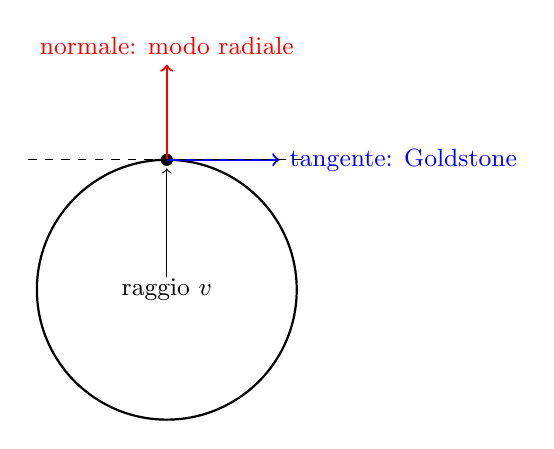
\begin{tikzpicture}[scale=1.1]
\draw[thick] (0,0) circle (1.5);
\fill (0,1.5) circle (2pt);
\draw[->,thick,blue] (0,1.5)--(1.3,1.5) node[right]{\small tangente: Goldstone};
\draw[->,thick,red] (0,1.5)--(0,2.6) node[above]{\small normale: modo radiale};
\draw[dashed] (-1.6,1.5)--(1.6,1.5);
\node at (0,0) {\small raggio $v$};
\draw[->] (0,0.15)--(0,1.4);
\end{tikzpicture}
\end{center}

Pensa a un cerchio di raggio $v$ disegnato nel piano. Ci sono due modi di parlare della sua curvatura:
\begin{itemize}
\item \textbf{Curvatura estrinseca:} quanto rapidamente il cerchio si allontana dalla sua retta tangente, vista dal piano in cui è immerso. Vale $1/v$. Per definirla serve lo spazio esterno (il piano) e la direzione \emph{normale} (rossa).
\item \textbf{Curvatura intrinseca:} quella che misurerebbe un essere che vive \emph{sulla} superficie senza poter guardare fuori. Per una curva è zero (una curva è sempre ``piatta'' dall'interno), ma per una superficie come la sfera no. La sfera $S^2$ di raggio $v$ ha curvatura intrinseca $1/v^2$: la somma degli angoli di un triangolo disegnato sulla sfera supera $\pi$.
\end{itemize}
Il \textbf{teorema di Gauss} (\emph{Theorema Egregium}) dice che, per una superficie immersa in uno spazio piatto, la curvatura intrinseca è il prodotto delle curvature estrinseche. Per la sfera: $\frac1{v^2}=\frac1v\cdot\frac1v$.

\subsection{Traduzione nel linguaggio dei campi}

\begin{center}
\begin{tabular}{p{0.42\textwidth}p{0.5\textwidth}}
\hline
geometria & fisica\\
\hline
spazio piatto ambiente & spazio dei campi lineari $\phi$ (teoria rinormalizzabile)\\
superficie & varietà dei vuoti, il coset $\G/\Hg$\\
direzioni tangenti & Goldstone $\pi^a$\\
direzioni normali & modi radiali $\rho^r$\\
curvatura intrinseca & crescita dell'ampiezza del NL$\Sigma$M\\
curvatura estrinseca (seconda forma fondamentale) & accoppiamenti $g^r_{ab}$ dei modi radiali ai $\pi\pi$\\
teorema di Gauss & cancellazione della crescita\\
\hline
\end{tabular}
\end{center}

\textbf{Perché la crescita del NL$\Sigma$M è la curvatura intrinseca.} Il NL$\Sigma$M conosce solo la metrica $g_{ab}(\pi)$ del coset. Vicino al vuoto, in coordinate opportune (``normali''), una metrica si scrive sempre come $g_{ab}=\delta_{ab}-\frac13R_{acbd}\pi^c\pi^d+\dots$, dove $R$ è il tensore di Riemann (la curvatura). Il termine con $R$ è esattamente un'interazione $\pi\pi\partial\pi\partial\pi$, cioè il contatto a quattro Goldstone. Se lo spazio fosse piatto ($R=0$) non ci sarebbero interazioni e nessuna crescita. Dunque: \emph{la crescita dell'ampiezza dei Goldstone è la curvatura del coset}.

\textbf{Perché gli accoppiamenti radiali sono la curvatura estrinseca.} Se scrivi il campo lineare come ``punto sul coset + spostamento normale'', l'accoppiamento $\rho\,\partial\pi\partial\pi$ viene dalla derivata seconda dell'immersione proiettata sulla direzione normale. In altre parole, misura quanto la superficie si allontana dal piano tangente (lo rivedremo nel Cap.~\ref{cap:gauss}).

\subsection{Perché le sfere sono speciali}

Su una sfera tutte le direzioni sono equivalenti: la curvatura è la stessa in ogni piano (\emph{curvatura costante}). Per ``piegare'' una sfera dentro uno spazio piatto basta \emph{una} direzione normale, il raggio. Fisicamente basta un modo radiale singoletto, l'Higgs.

Un coset generico ha invece direzioni più curve e direzioni piatte. Il coset di $SU(3)\times SU(3)/SU(3)$ contiene piani ``piatti'' (quelli generati da due generatori che commutano) e piani curvi. Con una sola direzione normale, che piega allo stesso modo in tutte le direzioni, non si può riprodurre una curvatura che cambia da piano a piano. \emph{Servono più direzioni normali, cioè più modi radiali.} Questa è, in una riga, l'idea della Proposizione~2 del paper.

\begin{porta}
\begin{itemize}[nosep]
\item crescita del NL$\Sigma$M $=$ curvatura intrinseca del coset;
\item accoppiamenti radiali $=$ curvatura estrinseca, cioè il piegamento nello spazio dei campi;
\item la cancellazione è il teorema di Gauss;
\item sfera $\Rightarrow$ basta un modo radiale; coset con direzioni piatte $\Rightarrow$ ne servono di più.
\end{itemize}
\end{porta}

%=====================================================================
\section{La domanda del paper e la strategia}
\label{cap:domanda}
%=====================================================================

\begin{dove}
Ora sappiamo qual è il problema e abbiamo l'intuizione. Prima di entrare nei conti, fissiamo con precisione \emph{che cosa} vogliamo dimostrare e \emph{come}, così ogni sezione successiva ha uno scopo chiaro.
\end{dove}

\subsection{I tre coset}

Il paper considera i tre pattern di rottura delle teorie di gauge ``tipo QCD'', con $N$ fermioni in una rappresentazione del gruppo di gauge:
\begin{center}
\begin{tabular}{p{0.3\textwidth}p{0.3\textwidth}p{0.3\textwidth}}
\hline
fermioni in rappresentazione & pattern & esempio\\
\hline
complessa (come i quark di QCD) & $SU(N)\times SU(N)/SU(N)$ & QCD, technicolor\\
reale & $SU(N)/SO(N)$ & gauge $SO$ con fermioni vettoriali\\
pseudoreale & $SU(2N)/Sp(2N)$ & gauge $SU(2)$ o $Sp$: composite Higgs minimale\\
\hline
\end{tabular}
\end{center}
Per $N=2$ sono tutti sfere: $SU(2)\times SU(2)/SU(2)\simeq S^3$, $SU(2)/SO(2)\simeq S^2$, $SU(4)/Sp(4)\simeq S^5$. Quindi per $N=2$ basta un Higgs singoletto, come nel Cap.~\ref{cap:toy}. Per $N\ge3$ non sono sfere, e la domanda diventa interessante.

\subsection{La domanda, precisa}

\emph{Dato uno di questi coset con $N\ge3$, quali modi radiali deve contenere un completamento lineare? La risposta dipende dalla rappresentazione scelta?}

\subsection{Due approcci complementari}

\textbf{Approccio gruppale} (quello suggerito dal referee~A). Si cerca una rappresentazione di $\G$ che contenga una direzione invariante sotto $\Hg$ (dove mettere il vuoto) e in cui i NGB compaiano come direzioni tangenti. Si scrive il modello lineare con quella rappresentazione: per costruzione è rinormalizzabile, quindi ha ampiezze limitate.
\begin{itemize}[nosep]
\item \emph{Pro:} dà subito un completamento che funziona.
\item \emph{Contro:} non dice se tutti i modi radiali di quella rappresentazione sono davvero necessari, né se una rappresentazione diversa ne richiederebbe altri.
\end{itemize}

\textbf{Approccio dalle ampiezze} (quello del paper). Si parte dal NL$\Sigma$M, si scrive il modo più generale in cui dei modi radiali possono accoppiarsi ai Goldstone, e si impone che la crescita si cancelli. Si ottiene una condizione (l'equazione di Gauss) che \emph{ogni} completamento deve soddisfare, qualunque sia la rappresentazione.
\begin{itemize}[nosep]
\item \emph{Pro:} dà condizioni necessarie universali.
\item \emph{Contro:} da solo non costruisce un modello; una soluzione dell'equazione potrebbe non corrispondere a nessuna rappresentazione.
\end{itemize}
Il paper usa entrambi: il primo per costruire il modello ``standard'' (matriciale), il secondo per dire cosa è obbligatorio in generale.

\subsection{I risultati, in anticipo}

\begin{enumerate}
\item In ogni completamento serve un modo radiale singoletto (Prop.~1).
\item I soli singoletti bastano se e solo se il coset è una sfera, cioè $N=2$ (Prop.~2).
\item Nel modello matriciale i modi radiali sono un singoletto $h$ e un multipletto $H^a$ con gli stessi numeri quantici dei Goldstone, e servono tutti (Prop.~3).
\item Per $N=3$, \emph{qualunque} completamento deve contenere un multipletto come $H^a$ (Prop.~4). Per $N=4$ invece esistono completamenti che ne fanno a meno: sono i nuovi risultati.
\item Le masse dei modi radiali sono limitate dall'unitarietà, $m\lesssim\sqrt{4\pi/N}\,f$.
\end{enumerate}

%=====================================================================
\section{L'equazione di Gauss dalle ampiezze, e le sue prime conseguenze}
\label{cap:gauss}
%=====================================================================

\begin{dove}
Generalizziamo il Cap.~\ref{cap:toy} a un completamento lineare \emph{qualsiasi}. È il cuore concettuale del paper (Sez.~II.B--C): da qui escono le Proposizioni 1 e 2, valide per qualunque rappresentazione. Non serve ancora sapere nulla sui tre coset specifici.
\end{dove}

\subsection{Impostazione}

Prendiamo campi reali $\phi$ in una rappresentazione di $\G$, con Lagrangiana $\frac12(\partial\phi)^2-V(\phi)$ e un vuoto $v$ invariante sotto $\Hg$. Come nel Cap.~\ref{cap:toy} usiamo coordinate polari, che ora hanno questa forma:
\[
\phi=U(\pi)\,(v+\rho),\qquad U(\pi)=e^{\pi^at_a/f}.
\]
\begin{itemize}
\item $U(\pi)$ è una trasformazione di simmetria rotta: muove il vuoto \emph{lungo} la varietà dei vuoti. È il ``punto sulla sfera'' del Cap.~\ref{cap:toy}.
\item $\rho$ è uno spostamento nelle direzioni \emph{perpendicolari} alla varietà dei vuoti: sono i modi radiali, l'analogo di $h$.
\item $t_a$ sono i generatori rotti nella rappresentazione di $\phi$ (matrici reali antisimmetriche). I vettori $t_av$ sono le direzioni tangenti; li normalizziamo con $(t_av)\cdot(t_bv)=f^2\delta_{ab}$, così che i $\pi$ abbiano termine cinetico canonico.
\end{itemize}

\subsection{Gli accoppiamenti dei modi radiali}

\textbf{Perché facciamo questo conto.} Vogliamo l'analogo del termine $\frac1vh(\partial\pi)^2$ della \eqref{eq:toypolar}, cioè l'accoppiamento $\rho\,\partial\pi\partial\pi$, per un modello qualsiasi.

Deriviamo: $\partial\phi=U\big[(U^{-1}\partial U)(v+\rho)+\partial\rho\big]$ e, al primo ordine, $U^{-1}\partial U\simeq\frac{\partial\pi^a}{f}t_a$. Il termine cinetico $\frac12|\partial\phi|^2$ contiene allora:
\begin{enumerate}
\item $\frac{1}{2f^2}\partial\pi^a\partial\pi^b(t_av)\cdot(t_bv)=\frac12(\partial\pi)^2$, il termine cinetico dei Goldstone;
\item un termine misto $\partial\rho\cdot t_av$, che è zero perché $\rho$ è perpendicolare ai $t_av$;
\item il termine con un $\rho$ e due $\partial\pi$: $\frac{1}{f^2}\partial\pi^a\partial\pi^b(t_av)\cdot(t_b\rho)$.
\end{enumerate}
Il terzo termine è quello che cercavamo. Usando l'antisimmetria $t^T=-t$ e simmetrizzando in $a,b$:
\begin{equation}
\mathcal L\supset\frac1f\,g^r_{ab}\,\rho^r\partial\pi^a\partial\pi^b,\qquad g^r_{ab}=-\frac{1}{2f}\,n_r\cdot\{t_a,t_b\}v .
\end{equation}
\textbf{Interpretazione.} $\{t_a,t_b\}v$ è la derivata seconda di $U(\pi)v$ rispetto ai $\pi$. $n_r\cdot(\ldots)$ ne prende la componente normale, cioè quanto la varietà dei vuoti si allontana dal piano tangente nella direzione $r$. È la curvatura estrinseca del Cap.~\ref{cap:geo}, che i geometri chiamano \emph{seconda forma fondamentale}.

\textbf{Controllo sul giocattolo.} Per la sfera c'è una sola direzione normale ($h$) e $g_{ab}=\delta_{ab}$, che riproduce l'accoppiamento $\frac1vh(\partial\pi)^2$ con $f=v$.

\subsection{Le ampiezze}

\textbf{Perché ci serve.} Vogliamo imporre che la crescita si cancelli, come nel Cap.~\ref{cap:toy}.

Il NL$\Sigma$M dà un contatto che cresce. Lo calcoleremo nel Cap.~\ref{cap:ccwz}; il risultato è
\begin{equation}
\mathcal A_{\rm NL\Sigma M}=-\frac{1}{f^2}\Big[t\,F^{adbc}+u\,F^{acbd}\Big],\qquad F^{abcd}\equiv f^{abI}f^{cdI},
\end{equation}
dove le $f^{abI}$ sono le costanti di struttura (i commutatori dei generatori rotti). $F$ è la curvatura del coset. Per la sfera $F^{abcd}=\delta_{ac}\delta_{bd}-\delta_{ad}\delta_{bc}$, e si ritrova $A=s/v^2$.

Lo scambio di un modo radiale $\rho^r$ dà, esattamente come per l'Higgs del Cap.~\ref{cap:toy} con $1/v\to g^r_{ab}/f$:
\[
\mathcal A_\rho=-\frac1{f^2}\sum_r\Big[g^r_{ab}g^r_{cd}\frac{s^2}{s-m_r^2}+g^r_{ac}g^r_{bd}\frac{t^2}{t-m_r^2}+g^r_{ad}g^r_{bc}\frac{u^2}{u-m_r^2}\Big].
\]
Ad alte energie $\frac{s^2}{s-m^2}\simeq s+m^2$: ogni scambio cresce come $s$, come nel giocattolo.

\subsection{Imporre la cancellazione}

Chiamiamo $G^{ab,cd}=\sum_rg^r_{ab}g^r_{cd}$. La parte che cresce dell'ampiezza totale è
\[
\frac{1}{f^2}\Big[-tF^{adbc}-uF^{acbd}\Big]-\frac1{f^2}\Big[sG^{ab,cd}+tG^{ac,bd}+uG^{ad,bc}\Big].
\]
\textbf{Il trucco:} $s$, $t$, $u$ non sono indipendenti ($s=-t-u$). Sostituisco $s$; restano $t$ e $u$ indipendenti, quindi i loro coefficienti devono annullarsi separatamente. Questo dà due equazioni, che con un po' di algebra (e la simmetria $F^{acbd}=F^{abcd}+F^{adbc}$, identità di Bianchi) risultano equivalenti a una sola:
\begin{equation}
\boxed{\;f^{abI}f^{cdI}=\sum_r\Big(g^r_{ac}g^r_{bd}-g^r_{ad}g^r_{bc}\Big)\;}
\label{eq:gauss}
\end{equation}
È l'\textbf{equazione di Gauss}: a sinistra la curvatura intrinseca, a destra quella estrinseca. Vale per \emph{qualunque} completamento lineare, perché nel conto non abbiamo mai usato la rappresentazione specifica.

\textbf{Perché è garantito che valga in un vero modello lineare?} In coordinate cartesiane non ci sono derivate e le ampiezze sono limitate; cambiare coordinate nei campi non cambia le ampiezze. Quindi in un modello lineare vero l'equazione di Gauss vale automaticamente. Usata ``al contrario'', ci dice cosa \emph{deve} avere un modello per funzionare.

\subsection{Conseguenza 1: il singoletto è sempre necessario}

\textbf{Domanda.} Si può completare il coset senza un modo radiale singoletto, cioè invariante sotto $\Hg$?

\textbf{Idea.} Prendiamo la ``traccia'' dell'equazione di Gauss, contraendo $a=c$ e $b=d$. A sinistra viene la \emph{curvatura scalare} $\sum f^{abI}f^{abI}$, che è positiva perché è una somma di quadrati. A destra si scopre che solo i singoletti danno un contributo positivo; i multipletti non banali contribuiscono con segno negativo o zero.

\textbf{Perché solo i singoletti.} Un accoppiamento $g^r_{ab}$ di un singoletto deve essere invariante, e l'unica matrice invariante è $\delta_{ab}$ (lemma di Schur). Per un multipletto non banale, invece, la traccia $\sum_a g^r_{aa}$ deve essere nulla, perché è un numero invariante costruito con un oggetto non invariante.

\textbf{Il conto.} Con $g^r=\frac{\Tr g^r}{D}\one+\hat g^r$ (parte di traccia più parte senza traccia):
\[
\sum f^{abI}f^{abI}=\sum_r\Big[\frac{D-1}{D}(\Tr g^r)^2-\Tr(\hat g^r)^2\Big]\le D(D-1)\sum_{\rm singoletti}g_r^2 .
\]
Quindi
\begin{equation}
\sum_{\rm singoletti}g_r^2\ \ge\ \bar K\equiv\frac{\sum f^{abI}f^{abI}}{D(D-1)}\ >\ 0 .
\end{equation}
$\bar K$ è la curvatura \emph{media} del coset. Senza singoletti la disuguaglianza è impossibile.

\textbf{Intuizione.} Il coset è curvo ``in media'' e solo una direzione normale invariante può dare questa curvatura media positiva. Nel giocattolo, il singoletto è l'Higgs.

\subsection{Conseguenza 2: solo singoletti $\iff$ sfera}

\textbf{Domanda.} Bastano i singoletti?

\textbf{Idea.} Se ci sono solo singoletti, $g^r_{ab}=g_r\delta_{ab}$, e la destra della \eqref{eq:gauss} diventa $(\sum g_r^2)(\delta_{ac}\delta_{bd}-\delta_{ad}\delta_{bc})$. È una curvatura uguale in ogni piano, cioè quella di una sfera. Quindi i singoletti bastano solo se il coset ha curvatura costante.

\textbf{Perché per $N\ge3$ i nostri coset non hanno curvatura costante.} Per $N\ge3$ esistono due generatori rotti che commutano, per esempio due matrici diagonali come $\mathrm{diag}(1,-1,0)$ e $\mathrm{diag}(1,1,-2)$. Per loro $f^{abI}=0$: il piano che generano è \emph{piatto} (curvatura zero). Altre coppie non commutano e danno curvatura positiva. Una curvatura che vale zero in un piano e un valore positivo in un altro non è costante. (Il numero massimo di generatori rotti che commutano tra loro si chiama \emph{rango}; per i nostri coset vale $N-1$, quindi ci sono piani piatti appena $N\ge3$.)

\begin{porta}
\begin{itemize}[nosep]
\item L'equazione di Gauss \eqref{eq:gauss} è la condizione universale per cancellare la crescita.
\item Serve sempre un singoletto, con accoppiamento almeno pari alla curvatura media.
\item Per $N\ge3$ servono anche multipletti non singoletti, qualunque sia la rappresentazione.
\item Resta da capire \emph{quali} multipletti: lo vedremo nei Capp.~\ref{cap:lineare}--\ref{cap:rigid}.
\end{itemize}
\end{porta}

%=====================================================================
\section{Gli strumenti di teoria dei gruppi per i tre coset}
\label{cap:gruppi}
%=====================================================================

\begin{dove}
Fin qui tutto era generale. Per dire qualcosa di concreto sui tre coset ci servono i loro generatori, le loro proprietà, e la struttura ``simmetrica'' che li accomuna. Nel paper è l'inizio della Sez.~II e la Sez.~III.
\end{dove}

\subsection{Generatori rotti e non rotti}

L'algebra di Lie di $\G$ si divide in due parti:
\begin{itemize}[nosep]
\item $\h$: i generatori $T^I$ che lasciano invariato il vuoto (non rotti);
\item $\p$: i generatori rotti $X^a$, uno per ogni Goldstone.
\end{itemize}
Normalizziamo tutto con $\Tr(XX)=\frac12$, come i $\lambda/2$ di Gell-Mann.

\textbf{Esempi espliciti} (questi ti conviene averli sempre davanti):
\begin{center}
\begin{tabular}{p{0.2\textwidth}p{0.4\textwidth}p{0.3\textwidth}}
\hline
coset & generatori rotti $X^a$ (cioè $\p$) & generatori non rotti $T^I$ (cioè $\h$)\\
\hline
$SU(N)\times SU(N)/SU(N)$ & tutte le Hermitiane a traccia nulla & idem (agiscono in modo diverso)\\
$SU(N)/SO(N)$ & reali simmetriche a traccia nulla & immaginarie antisimmetriche\\
$SU(2N)/Sp(2N)$ & Hermitiane con $X^T\Omega=\Omega X$ & Hermitiane con $T^T\Omega=-\Omega T$\\
\hline
\end{tabular}
\end{center}
Qui $\Omega=\begin{pmatrix}0&\one\\-\one&0\end{pmatrix}$ è la matrice simplettica.

\textbf{Esempio con $SU(3)/SO(3)$.} Le 8 matrici di Gell-Mann si dividono in 3 immaginarie antisimmetriche ($\lambda_2,\lambda_5,\lambda_7$: generano $SO(3)$) e 5 reali simmetriche ($\lambda_1,\lambda_3,\lambda_4,\lambda_6,\lambda_8$: i 5 Goldstone).

\textbf{Il caso chirale.} I generatori rotti sono $(T,-T)$, cioè $L$ e $R$ ruotano in direzioni opposte (rotazioni assiali); i non rotti sono $(T,T)$, rotazioni vettoriali.

\subsection{Coset simmetrici: la ``parità'' dei Goldstone}

Tutti e tre i coset hanno una proprietà in comune: il commutatore di due generatori rotti è un generatore non rotto,
\begin{equation}
[X^a,X^b]=i f^{abI}\,T^I\quad\in\h .
\end{equation}
Si dice che il coset è \emph{simmetrico}. Equivalentemente esiste una ``parità'' $\mathcal R$ che lascia fissi i $T$ e cambia segno agli $X$, cioè $\pi\to-\pi$ sui Goldstone. Nel caso chirale è lo scambio $L\leftrightarrow R$; per $SO$ è la coniugazione complessa.

\textbf{Perché ci interessa.} (i) Le $f^{abI}$ di questo commutatore sono proprio quelle che compaiono nella curvatura $F=ff$. (ii) Quando, nel Cap.~\ref{cap:lineare}, faremo un \emph{anticommutatore} di due $X$, scopriremo che resta dentro gli $X$ (più l'identità): è la proprietà ``gemella'', da cui nasce tutto.

\textbf{Verifica nel caso $SO$.} Se $X$, $Y$ sono reali simmetriche, $[X,Y]$ è reale antisimmetrica, cioè $i\times$(immaginaria antisimmetrica), che è un generatore di $SO(N)$. \checkmark

\subsection{Rango: le direzioni piatte}

Il rango è il massimo numero di generatori rotti che commutano tra loro. Per i tre coset è $N-1$: sono le matrici diagonali (per $Sp$, della forma $\mathrm{diag}(\Lambda,\Lambda)$). Questo è il fatto usato nella Prop.~2: per $N\ge3$ ci sono almeno due direzioni rotte che commutano, quindi un piano piatto.

\subsection{Il $U(1)$ e il bosone $\eta$}

Il paper aggiunge un $U(1)$ globale, sotto cui il campo lineare ha carica 1. Rompendolo nasce un Goldstone in più, $\eta$, associato al generatore $X^0=\one/\sqrt{2n}$ ($n$ è la taglia delle matrici: $N$, $N$, $2N$). È comodo trattare $\eta$ insieme agli altri con un indice $A=0,1,\dots,D$. Poiché $X^0$ commuta con tutto, $f^{0BI}=0$: nel NL$\Sigma$M l'$\eta$ è libero.

\begin{attento}
Nella v1: $\dim Sp(2N)=N(2N+1)$, non $N(N+1)/2-1$. I Goldstone di $SU(2N)/Sp(2N)$ sono $2N^2-N-1$ (5 per $N=2$, come $SO(6)/SO(5)$).
\end{attento}

\begin{porta}
\begin{itemize}[nosep]
\item $[X,X]\subset\h$ (coset simmetrico): dà le $f^{abI}$, cioè la curvatura.
\item Rango $N-1$: piani piatti per $N\ge3$.
\item Il $U(1)$ aggiunge l'$\eta$, con $X^0\propto\one$.
\end{itemize}
\end{porta}

%=====================================================================
\section{La costruzione CCWZ: come si scrive il NL$\Sigma$M}
\label{cap:ccwz}
%=====================================================================

\begin{dove}
Abbiamo usato l'ampiezza del NL$\Sigma$M senza ricavarla. Ora la ricaviamo, e introduciamo gli oggetti $d_\mu$ ed $E_\mu$ che serviranno per la Lagrangiana del modello lineare (Cap.~\ref{cap:lineare}). Nel paper è la Sez.~II.A.
\end{dove}

\subsection{Il problema: i Goldstone trasformano in modo non lineare}

Sotto la simmetria $\G$ i Goldstone non si trasformano come una rappresentazione lineare: nel giocattolo, una rotazione che sposta il vuoto rimescola $\pi$ e $\sqrt{v^2-\pi^2}$. Per scrivere Lagrangiane invarianti serve un metodo sistematico. È la costruzione CCWZ (Callan, Coleman, Wess, Zumino).

\textbf{La ricetta.}
\begin{enumerate}
\item Si mettono i Goldstone in una matrice $u(\pi)=e^{i\pi^aX^a/f}$, che rappresenta ``il punto sul coset''.
\item Sotto $g\in\G$, $g\,u$ è in generale un elemento qualsiasi di $\G$, ma lo si può riscrivere come $u(\pi')\,k$ con $k\in\Hg$. Quindi $u\to g\,u\,k^{-1}$. La $k$ (compensatore) dipende da $\pi$, ed è qui che sta la non linearità.
\item Si costruisce $u^{-1}\partial_\mu u$, che sta nell'algebra di Lie, e lo si spezza in parte rotta e parte non rotta:
\begin{equation}
u^{-1}\partial_\mu u=i\big(d_\mu+E_\mu\big),\qquad d_\mu\in\p,\quad E_\mu\in\h .
\end{equation}
\end{enumerate}
\textbf{Significato.} $d_\mu$ è la ``velocità'' sul coset: trasforma semplicemente, $d\to k\,d\,k^{-1}$. $E_\mu$ è una ``connessione'', come un campo di gauge, che serve per costruire derivate covarianti.

\subsection{Sviluppo esplicito}

\textbf{Perché ci serve.} Per ottenere l'interazione a quattro Goldstone dobbiamo sviluppare $d_\mu$ fino al terzo ordine nei campi.

Con $A=\pi\cdot X/f$, la formula generale $e^{-iA}\partial e^{iA}=i\partial A+\frac12[A,\partial A]-\frac i6[A,[A,\partial A]]+\dots$ (si ottiene sviluppando gli esponenziali) dà, separando $\p$ e $\h$ con la regola $[\p,\p]\subset\h$:
\[
d_\mu=\partial_\mu A-\tfrac16[A,[A,\partial_\mu A]]+\dots,\qquad E_\mu=-\tfrac i2[A,\partial_\mu A]+\dots
\]

\subsection{La Lagrangiana e il vertice a quattro Goldstone}

La Lagrangiana invariante più semplice è $\mathcal L=f^2\Tr(d_\mu d^\mu)$: è invariante perché $d\to kdk^{-1}$ e la traccia non cambia. Sviluppando:
\begin{itemize}
\item al secondo ordine viene $\frac12(\partial\pi)^2$, il termine cinetico canonico (è per questo che si mette $f^2$ davanti);
\item al quarto ordine, con un po' di algebra di commutatori, viene
\begin{equation}
\mathcal L_4=-\frac{1}{6f^2}\,f^{abI}f^{cdI}\,\pi^a\partial\pi^b\,\pi^c\partial\pi^d .
\end{equation}
\end{itemize}
\textbf{Controllo.} Per $SU(2)$, $f^{abI}=\epsilon^{abI}$, e si ritrova la Lagrangiana chirale standard dei pioni. \checkmark

\textbf{Dal vertice all'ampiezza.} Si sommano i 24 modi di attaccare le quattro gambe esterne. Si usano le relazioni tra prodotti scalari e $s,t,u$ ($p_1\cdot p_2=s/2$ ecc.) e l'identità di Bianchi. Si ottiene
\begin{equation}
\mathcal A_{\rm NL\Sigma M}(\pi^a\pi^b\to\pi^c\pi^d)=-\frac{1}{f^2}\Big[t\,f^{adI}f^{bcI}+u\,f^{acI}f^{bdI}\Big],
\end{equation}
che per $SU(2)$ è la formula di Weinberg $A=s/f^2$. Il conto passo per passo è nel formulario \texttt{notes.pdf}, Sez.~6.

\begin{porta}
\begin{itemize}[nosep]
\item CCWZ: $u=e^{i\pi X/f}$, e $u^{-1}\partial u=i(d+E)$ con $d$ covariante ed $E$ connessione.
\item $\mathcal L=f^2\Tr d^2$; il contatto a quattro Goldstone è $\propto ff$, la curvatura.
\item $d$ ed $E$ torneranno nella Lagrangiana del modello lineare.
\end{itemize}
\end{porta}

%=====================================================================
\section{Il modello lineare dei tre coset}
\label{cap:lineare}
%=====================================================================

\begin{dove}
Ora costruiamo il completamento lineare concreto (approccio gruppale): un campo matriciale $\Hf$ con un potenziale a cappello messicano. Scopriremo quali sono i suoi modi radiali, come si accoppiano, e scriveremo la Lagrangiana in una forma chiusa che ricorda da vicino il giocattolo. Nel paper sono le Sezz.~III e IV.
\end{dove}

\subsection{La scelta del campo}

Seguiamo l'approccio gruppale: serve una rappresentazione con un vuoto invariante sotto $\Hg$. La scelta più piccola è una matrice complessa:
\begin{center}
\begin{tabular}{llll}
\hline
coset & campo & come trasforma & vuoto\\
\hline
chirale & $\Hf$ matrice $N\times N$ qualsiasi & $\Hf\to L\Hf R^\dagger$ & $\propto\one$\\
$SO$ & $\Hf=\Hf^T$ (simmetrica) & $\Hf\to V\Hf V^T$ & $\propto\one$\\
$Sp$ & $\Hf=-\Hf^T$ (antisimmetrica) & $\Hf\to V\Hf V^T$ & $\propto\Omega$\\
\hline
\end{tabular}
\end{center}
\textbf{Verifica dei vuoti.} $L\one R^\dagger=\one$ vale se e solo se $L=R$: resta $SU(N)_V$. $V\one V^T=\one$ vale se e solo se $V$ è ortogonale: resta $SO(N)$. $V\Omega V^T=\Omega$ vale se e solo se $V$ è simplettica: resta $Sp(2N)$.

\textbf{Conteggio.} Il campo ha $D_\R$ componenti reali, per esempio $2N^2$ nel caso chirale. Togliendo i $D+1$ Goldstone ($\pi^a$ ed $\eta$) restano esattamente $D+1$ modi radiali: tanti quanti i Goldstone. Non è una coincidenza, e il motivo è nella prossima sottosezione.

\subsection{L'osservazione chiave: i modi radiali sono anticommutatori}

\textbf{Perché questo è il punto centrale.} Nel Cap.~\ref{cap:gauss} abbiamo visto che gli accoppiamenti radiali sono la ``derivata seconda'' dell'orbita del vuoto. Calcoliamola esplicitamente per il caso chirale e vediamo che cosa esce.

L'orbita del vuoto è $\Hf\propto u^2=e^{2iA}$, con $A=\pi\cdot X/f$ Hermitiana. Sviluppando:
\[
e^{2iA}=\one+\underbrace{2iA}_{\text{1° ordine}}\;\underbrace{-\,2A^2}_{\text{2° ordine}}+\dots
\]
\begin{itemize}
\item Il primo ordine, $2iA$, è $i\times$(Hermitiana): sono le \textbf{direzioni tangenti}, cioè i Goldstone. I Goldstone vivono nella ``parte immaginaria'' di $\Hf$.
\item Il secondo ordine, $-2A^2$, è \textbf{Hermitiano}, quindi perpendicolare alle direzioni tangenti: è la direzione in cui l'orbita si piega, cioè i \textbf{modi radiali}. I modi radiali vivono nella ``parte reale'' (Hermitiana) di $\Hf$.
\end{itemize}
Ora scriviamo $A^2$ con i generatori: $A^2=\frac{1}{f^2}\pi^a\pi^bX^aX^b=\frac{1}{2f^2}\pi^a\pi^b\{X^a,X^b\}$. Gli accoppiamenti radiali sono quindi dati dall'\textbf{anticommutatore} $\{X^a,X^b\}$.

Per le matrici Hermitiane l'anticommutatore di due generatori è di nuovo una combinazione di generatori più l'identità:
\begin{equation}
\{X^a,X^b\}=\frac1n\delta^{ab}\one+d^{abc}X^c .
\label{eq:jordan}
\end{equation}
\begin{itemize}
\item La parte $\propto\one$ dice che i Goldstone si accoppiano a un modo radiale singoletto $h$, con forza $\propto\delta^{ab}$.
\item La parte $d^{abc}X^c$ dice che si accoppiano a un multipletto radiale $H^c$, con gli stessi indici dei generatori, cioè gli stessi numeri quantici dei Goldstone, con forza $d^{abc}$.
\end{itemize}

\textbf{La proprietà che rende tutto possibile.} Nei tre coset vale:
\begin{center}
\fbox{\parbox{0.85\textwidth}{\centering commutatore di due generatori rotti $\in$ generatori non rotti (coset simmetrico)\\[2pt]
anticommutatore di due generatori rotti $\in$ generatori rotti $+$ identità (algebra di Jordan)}}
\end{center}
La seconda riga si verifica a mano. Caso $SO$: l'anticommutatore di due reali simmetriche è reale simmetrico. Caso $Sp$: se $X^T\Omega=\Omega X$ e $Y^T\Omega=\Omega Y$, allora $\{X,Y\}^T\Omega=\Omega\{X,Y\}$. Uno spazio di matrici chiuso sotto anticommutatore si chiama \emph{algebra di Jordan}. Qui sono le matrici Hermitiane su reali, complessi e quaternioni.

\textbf{Il caso $N=2$.} Per matrici $2\times2$ (anche quaternioniche) ogni generatore a traccia nulla ha quadrato proporzionale all'identità: per esempio $\sigma_i^2=\one$. Quindi $\{X^a,X^b\}\propto\delta^{ab}\one$, cioè $d^{abc}=0$: il multipletto $H$ non si accoppia ai $\pi\pi$, e basta il singoletto. È l'origine algebrica del fatto che $N=2$ è una sfera.

\subsection{La parametrizzazione polare}

\textbf{Perché ci serve.} Vogliamo una parametrizzazione che separi nettamente Goldstone e modi radiali, come ``$(v+h)\,\vec n(\pi)$'' nel giocattolo. La versione matriciale è
\begin{equation}
\sqrt2\,\Hf=u\,\Phi\,u\ (\text{chirale}),\qquad u\,\Phi\,u^T\ (SO),\qquad u\,\Phi\,\Omega\,u^T\ (Sp),
\end{equation}
con $u=e^{i\pi\cdot X/f}$ (i Goldstone, la ``direzione'') e $\Phi$ Hermitiana (i modi radiali, il ``raggio''):
\begin{equation}
\Phi=\Big(f+\sqrt{\tfrac2n}\,h\Big)\one+2H^aX^a .
\end{equation}
È la versione matriciale della decomposizione polare di un numero complesso, $z=e^{i\theta}r$. I fattori $\sqrt{2/n}$ e $2$ servono a dare a $h$ e $H$ termini cinetici canonici. Nel vuoto $\Phi=f\one$.

\textbf{La parità diventa evidente.} $\pi\to-\pi$ manda $u\to u^\dagger$ e lascia $\Phi$ fermo, quindi $\Hf\to\Hf^\dagger$ (o $\Hf^*$). È una simmetria della Lagrangiana del modello lineare, e dunque non può generare vertici con un numero dispari di Goldstone. La v1 usava $\Hf=\Sigma\phi$, che nascondeva questa simmetria: è il punto 4 del referee~A.

\subsection{La Lagrangiana in forma chiusa}

Inserendo la parametrizzazione nella Lagrangiana $\frac12\Tr(\partial\Hf^\dagger\partial\Hf)-V$ e usando $d$ ed $E$ del Cap.~\ref{cap:ccwz}, si ottiene esattamente, a tutti gli ordini:
\begin{equation}
\boxed{\;\mathcal L=\underbrace{\tfrac14\Tr\big[(\nabla_\mu\Phi)^2\big]}_{\text{cinetico dei modi radiali}}+\underbrace{\tfrac14\Tr\big[\{d_\mu,\Phi\}^2\big]}_{\text{Goldstone con ``raggio'' }\Phi}-V(\Phi)\;}
\label{eq:master}
\end{equation}
dove $\nabla\Phi=\partial\Phi+i[E,\Phi]$.

\textbf{Confronto con il giocattolo.} Nel Cap.~\ref{cap:toy} avevamo $\frac12(\partial h)^2+\frac12(v+h)^2(\partial\vec n)^2$. Qui il primo termine è l'analogo di $\frac12(\partial h)^2$, il secondo è l'analogo di $\frac12(v+h)^2(\partial n)^2$, con il ``raggio'' $v+h$ promosso a matrice $\Phi$. Se $\Phi=f\one$ resta $f^2\Tr d^2$, cioè il NL$\Sigma$M.

\textbf{Come si ottiene} (idea della dimostrazione). Si deriva $\Hf$, si porta fuori la $u$ e si usa $u^{-1}\partial u=i(d+E)$. Le regole di trasposizione per $\p$ e $\h$ fanno combinare tutto in $i\{d,\Phi\}+\nabla\Phi$. I due pezzi sono Hermitiani, quindi nella traccia il termine misto si cancella. Il potenziale dipende solo da $\Phi$, perché $\Hf^\dagger\Hf\propto u^{-1}\Phi^2u$. Il conto riga per riga è nel formulario, Sez.~12.

\subsection{Gli accoppiamenti cubici}

Sviluppando $\frac14\Tr\{d,\Phi\}^2$ al primo ordine nei modi radiali:
\begin{equation}
\mathcal L_3=\frac1f\sqrt{\frac2n}\,h\,\big[(\partial\pi^a)^2+(\partial\eta)^2\big]+\frac1f\,d^{abc}\,H^c\,\partial\pi^a\partial\pi^b+\frac2f\sqrt{\frac2n}\,H^a\,\partial\pi^a\partial\eta .
\end{equation}
È esattamente quanto anticipato dall'anticommutatore. Per $n=2$ il primo termine è $\frac1f h(\partial\pi)^2$, l'accoppiamento dell'Higgs del giocattolo con $f=v$. \checkmark

\subsection{Potenziale e masse}

Con $V=-\frac{\mu^2}{2}\Tr\Hf^\dagger\Hf+\frac{\lambda_1}4(\Tr\Hf^\dagger\Hf)^2+\frac{\lambda_2}{4}\Tr(\Hf^\dagger\Hf)^2$, il minimo è a $\Phi=f\one$ con $f^2=2\mu^2/(n\lambda_1+\lambda_2)$, e
\begin{equation}
m_h^2=(n\lambda_1+\lambda_2)f^2,\qquad m_H^2=\lambda_2f^2 .
\end{equation}
\textbf{Interpretazione.}
\begin{itemize}
\item $\lambda_1$ (traccia doppia) tratta tutte le componenti allo stesso modo: tocca solo il singoletto.
\item $\lambda_2$ (traccia singola) distingue le direzioni: dà massa al multipletto.
\item Serve $\lambda_2>0$ perché il vuoto sia $\propto\one$; con $\lambda_2<0$ il vuoto si orienta diversamente.
\item Se $\lambda_2=0$ il potenziale ha una simmetria più grande e $H$ diventa senza massa (pseudo-Goldstone).
\end{itemize}

\begin{porta}
\begin{itemize}[nosep]
\item Goldstone $=$ parte ``immaginaria'' di $\Hf$; modi radiali $=$ parte ``reale'' (Hermitiana).
\item Gli accoppiamenti radiali sono anticommutatori di generatori: singoletto $h$ (forza $\sqrt{2/n}$) e multipletto $H$ (forza $d^{abc}$).
\item La Lagrangiana chiusa \eqref{eq:master} è la versione matriciale di $\frac12(\partial h)^2+\frac12(v+h)^2(\partial n)^2$.
\item Per $N=2$, $d^{abc}=0$: si torna al giocattolo.
\end{itemize}
\end{porta}

%=====================================================================
\section{Il cuore della dimostrazione: commutatori contro anticommutatori}
\label{cap:cuore}
%=====================================================================

\begin{dove}
Abbiamo il modello e i suoi accoppiamenti. Ora dobbiamo verificare che la crescita si cancelli davvero, cioè che l'equazione di Gauss \eqref{eq:gauss} sia soddisfatta. È il punto 1 del referee~A, che voleva la dimostrazione esplicita per tutti e tre i coset. Nel paper è la Sez.~V.A, Lemma~1.
\end{dove}

\subsection{Che cosa bisogna dimostrare}

Nell'equazione di Gauss mettiamo gli accoppiamenti del modello: $g^h_{ab}=\sqrt{2/n}\,\delta_{ab}$ per il singoletto e $g^c_{ab}=d^{abc}$ per il multipletto. Dobbiamo dimostrare che
\begin{equation}
\underbrace{f^{abI}f^{cdI}}_{\text{commutatori}}=\underbrace{\frac2n\big(\delta^{ac}\delta^{bd}-\delta^{ad}\delta^{bc}\big)+d^{ace}d^{bde}-d^{ade}d^{bce}}_{\text{anticommutatori}} .
\label{eq:lemma}
\end{equation}
A sinistra ci sono i commutatori (curvatura intrinseca, la crescita del NL$\Sigma$M), a destra gli anticommutatori (curvatura estrinseca, gli scambi di $h$ e $H$). È il teorema di Gauss scritto con le matrici.

\subsection{L'idea della dimostrazione}

Esiste un'identità valida per \emph{quattro matrici qualsiasi}, che lega il prodotto di due commutatori a prodotti di anticommutatori. A quel punto basta usare le due proprietà del Cap.~\ref{cap:lineare}: il commutatore di due $X$ dà le $f$, l'anticommutatore dà le $d$.

\subsection{Passo 1: un'identità per matrici qualsiasi}

Per quattro matrici $a,b,c,d$:
\begin{equation}
\Tr\big(\{a,c\}\{b,d\}\big)-\Tr\big(\{a,d\}\{b,c\}\big)=-\Tr\big([a,b][c,d]\big).
\label{eq:traceid}
\end{equation}
\textbf{Verifica.} Si espandono entrambi i lati. A sinistra ci sono 8 tracce di prodotti di quattro matrici, a destra 4. Usando la ciclicità della traccia, $\Tr(abcd)=\Tr(bcda)$, si riducono tutte a poche ``parole'' cicliche diverse, e i due lati coincidono termine per termine (il dettaglio è nel formulario, Sez.~13).

\textbf{Perché è vera, intuitivamente.} $ab=\frac12([a,b]+\{a,b\})$: commutatori e anticommutatori sono due modi complementari di scomporre il prodotto. Un'identità che li lega deve esistere.

\subsection{Passo 2: si usa la struttura dei coset}

Metti $a,b,c,d=X^a,X^b,X^c,X^d$.
\begin{itemize}
\item Destra: $[X^a,X^b]=if^{abI}T^I$, quindi $-\Tr([X^a,X^b][X^c,X^d])=\frac12f^{abI}f^{cdI}$.
\item Sinistra: $\{X^a,X^c\}=\frac1n\delta^{ac}\one+d^{ace}X^e$, quindi $\Tr(\{X^a,X^c\}\{X^b,X^d\})=\frac1n\delta^{ac}\delta^{bd}+\frac12d^{ace}d^{bde}$.
\end{itemize}
Moltiplicando per 2 si ottiene esattamente la \eqref{eq:lemma}. \qed

\textbf{Perché vale per tutti e tre i coset insieme.} Abbiamo usato solo due fatti: il commutatore di due $X$ cade in $\h$, e l'anticommutatore cade in $\p$ più l'identità. Valgono in tutti e tre i casi, quindi la dimostrazione è una sola.

\subsection{L'ampiezza esatta}

Con la cancellazione dimostrata, si può scrivere l'ampiezza completa in forma chiusa. Usando $\frac{s^2}{s-m^2}=s+\frac{m^2s}{s-m^2}$, i pezzi ``$s$'' cancellano il NL$\Sigma$M e resta
\begin{equation}
\mathcal A=-\sum_E\frac{m_E^2}{f^2}\Big[d^{abE}d^{cdE}\frac{s}{s-m_E^2}+(t)+(u)\Big],
\end{equation}
dove la somma su $E$ include il singoletto ($E=0$, massa $m_h$) e il multipletto (massa $m_H$). Confronta con il giocattolo \eqref{eq:toyA}: $A=-\frac{m^2}{v^2}\frac{s}{s-m^2}$ ha esattamente la stessa forma. Ad alte energie l'ampiezza tende a una costante di ordine $m^2/f^2\sim\lambda$; a basse energie riproduce il NL$\Sigma$M.

\begin{attento}
\textbf{Cosa non andava nella v1.} La v1 sostituiva $d^{abe}d^{cde}$ con una combinazione di $\delta$ e fissava i coefficienti con delle contrazioni. È una media, non un'identità: è esatta solo per le sfere ($N=2$). Il ``risultato principale'' della v1 era quindi vero per definizione. La conclusione era giusta, ma la ragione vera è l'identità \eqref{eq:lemma}.
\end{attento}

\begin{porta}
\begin{itemize}[nosep]
\item Gauss per il modello matriciale $\Leftrightarrow$ un'identità tra commutatori e anticommutatori.
\item Dimostrazione: un'identità di traccia generale più le due proprietà dei coset.
\item L'ampiezza esatta ha la stessa forma di quella del giocattolo.
\end{itemize}
\end{porta}

%=====================================================================
\section{Quali modi radiali sono necessari}
\label{cap:quali}
%=====================================================================

\begin{dove}
Sappiamo che con tutti i modi radiali del modello la crescita si cancella. Ma servono davvero tutti? È la domanda originale del paper, ristretta al modello matriciale. Nel paper è la Sez.~V.B--C.
\end{dove}

\subsection{Il ragionamento}

Guarda di nuovo la \eqref{eq:lemma}. A destra ci sono due pezzi: quello di $h$, $\frac2n(\delta\delta-\delta\delta)$, e quello di $H$, $dd-dd$. Se togliamo uno dei due modi, quel pezzo manca e la crescita non si cancella più. Ci sono due casi:
\begin{itemize}
\item \textbf{Togliere $h$:} manca il singoletto, e per la Prop.~1 non si può.
\item \textbf{Togliere $H$:} resterebbe $f f=\frac2n(\delta\delta-\delta\delta)$, cioè curvatura costante, e per la Prop.~2 per $N\ge3$ non si può.
\item \textbf{Togliere solo una parte di $H$:} $H$ è un multipletto irriducibile, e toglierne una parte romperebbe la simmetria $\Hg$.
\end{itemize}
Quindi per $N\ge3$ servono tutti (Prop.~3).

\subsection{Il caso $N=2$ e la sottigliezza dell'$\eta$}

Per $N=2$, $d^{abc}=0$, il pezzo di $H$ è nullo, e $h$ da solo basta per $\pi\pi\to\pi\pi$. Però, se c'è anche l'$\eta$ (il Goldstone del $U(1)$), il multipletto $H$ si accoppia a $\pi\eta$ (termine $H^a\partial\pi^a\partial\eta$). Nel processo $\pi\eta\to\pi\eta$:
\begin{itemize}[nosep]
\item il NL$\Sigma$M non dà nulla, perché $\eta$ è libero;
\item lo scambio di $h$ nel canale $t$ cresce;
\item lo scambio di $H$ nei canali $s$ e $u$ cresce con segno opposto e cancella.
\end{itemize}
Quindi, con l'$\eta$, anche per $N=2$ $H$ serve dentro questa rappresentazione. Esiste però una rappresentazione più piccola e \emph{riducibile} (un vettore reale di $SO(4)$ più un singoletto complesso separato per l'$\eta$) che non ne ha bisogno. È un primo esempio del fatto che la rappresentazione minimale irriducibile non è necessariamente il completamento minimo.

\subsection{Gli altri processi}

L'ampiezza esatta vale per tutti i processi con quattro Goldstone, inclusi quelli con $\eta$. Per esempio, in $\pi\pi\to\eta\eta$ gli scambi di $h$ e $H$ si combinano in $\propto s+t+u=0$. Nei processi con modi radiali esterni ($\pi\pi\to hh$, \ldots) la crescita si cancella tra termini di contatto e scambio di Goldstone. La Tab.~II del paper riassume tutto.

\begin{porta}
Nel modello matriciale, per $N\ge3$, servono il singoletto e tutto il multipletto. La ragione è nelle Prop.~1 e 2, che non dipendono dal modello.
\end{porta}

%=====================================================================
\section{Oltre il modello matriciale: rigidità a $N=3$, libertà a $N=4$}
\label{cap:rigid}
%=====================================================================

\begin{dove}
Finora abbiamo parlato di \emph{un} modello, quello matriciale. Ma il referee chiedeva: con un'altra rappresentazione potrebbero servire modi radiali diversi? Le Prop.~1 e 2 dicono che servono un singoletto e qualche multipletto, ma non quale. Qui rispondiamo: per $N=3$ deve essere proprio il multipletto con i numeri quantici dei Goldstone; per $N=4$ no. Nel paper sono la Sez.~VI e la nuova sezione su $N=4$.
\end{dove}

\subsection{Riformulare Gauss come un problema di ``somme positive''}

\textbf{Osservazione.} Un multipletto radiale in una rappresentazione $R$ di $\Hg$ può accoppiarsi a una coppia di Goldstone $\pi^a\pi^b$ solo se $R$ compare nel prodotto simmetrico di due Goldstone, ${\rm Sym}^2(R_\pi)$ (la coppia $\pi^a\pi^b$ con $\partial\pi^a\cdot\partial\pi^b$ è simmetrica in $a,b$). Per $SU(3)$ con i Goldstone nell'ottetto: $\mathbf8\otimes_S\mathbf8=\mathbf1\oplus\mathbf8\oplus\mathbf{27}$. Quindi i modi radiali che contano possono stare solo nell'$\mathbf1$, nell'$\mathbf8$ o nel $\mathbf{27}$.

\textbf{La forma degli accoppiamenti è fissata dalla simmetria.} Per ogni rappresentazione $R$ c'è un solo modo invariante di accoppiare $R$ a $\pi\pi$ (i coefficienti di Clebsch--Gordan); si può scegliere solo la forza. Il contributo di $R$ al lato destro dell'equazione di Gauss è quindi
\[
c_R\times(\text{un tensore fisso }\mathcal T_R),\qquad c_R=\sum(\text{accoppiamenti})^2\ \ge0 .
\]
L'equazione di Gauss diventa
\begin{equation}
F=\sum_Rc_R\,\mathcal T_R,\qquad c_R\ge0 .
\label{eq:cone}
\end{equation}
\textbf{Il punto cruciale: i coefficienti sono positivi}, perché sono somme di quadrati. Un multipletto può contribuire solo con il proprio ``segno''.

\subsection{Il piano delle curvature}

I tensori invarianti con le simmetrie di una curvatura, per i nostri coset, si scrivono come combinazioni di due soli tensori: $A=\delta^{ac}\delta^{bd}-\delta^{ad}\delta^{bc}$ (la curvatura ``sferica'') e $F=f^{abI}f^{cdI}$ (quella vera del coset). Ogni $\mathcal T_R$ è quindi un punto in un piano con coordinate $(\alpha_R,\beta_R)$:
\[
\mathcal T_R=\alpha_R\,A+\beta_R\,F .
\]
L'equazione \eqref{eq:cone} chiede di raggiungere il punto $F=(0,1)$ con una combinazione a coefficienti \emph{positivi} dei vettori $\mathcal T_R$.

\begin{center}
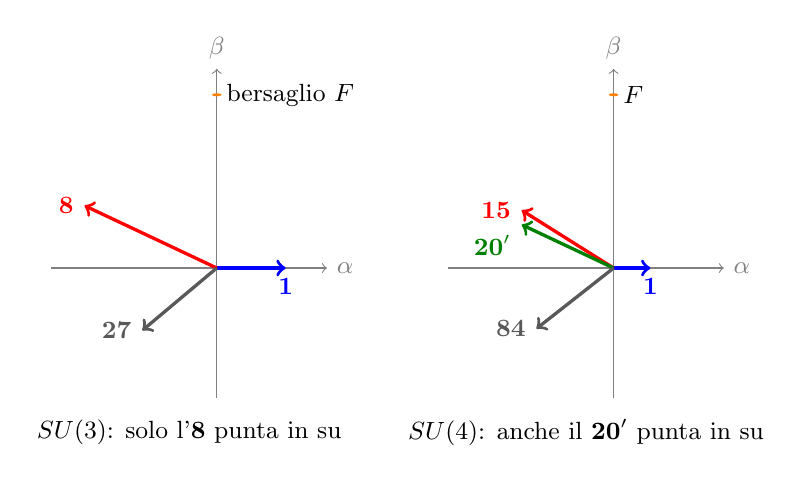
\begin{tikzpicture}[xscale=7,yscale=2.2]
% SU(3)
\begin{scope}
\draw[->,gray] (-0.3,0)--(0.2,0) node[right]{\small $\alpha$};
\draw[->,gray] (0,-0.75)--(0,1.15) node[above]{\small $\beta$};
\fill[orange] (0,1) circle (0.25pt) node[right,black]{\small bersaglio $F$};
\draw[->,very thick,blue] (0,0)--(0.125,0) node[below]{\small $\mathbf1$};
\draw[->,very thick,red] (0,0)--(-0.4*0.6,0.6*0.6) node[left]{\small $\mathbf8$};
\draw[->,very thick,gray!70!black] (0,0)--(-0.225*0.6,-0.6*0.6) node[left]{\small $\mathbf{27}$};
\node at (-0.05,-0.95) {\small $SU(3)$: solo l'$\mathbf8$ punta in su};
\end{scope}
\begin{scope}[shift={(0.72,0)}]
\draw[->,gray] (-0.3,0)--(0.2,0) node[right]{\small $\alpha$};
\draw[->,gray] (0,-0.75)--(0,1.15) node[above]{\small $\beta$};
\fill[orange] (0,1) circle (0.25pt) node[right,black]{\small $F$};
\draw[->,very thick,blue] (0,0)--(0.0667,0) node[below]{\small $\mathbf1$};
\draw[->,very thick,red] (0,0)--(-0.1667,0.3333) node[left]{\small $\mathbf{15}$};
\draw[->,very thick,green!50!black] (0,0)--(-0.1667,0.25) node[below left]{\small $\mathbf{20}'$};
\draw[->,very thick,gray!70!black] (0,0)--(-0.2333*0.6,-0.5833*0.6) node[left]{\small $\mathbf{84}$};
\node at (-0.05,-0.95) {\small $SU(4)$: anche il $\mathbf{20}'$ punta in su};
\end{scope}
\end{tikzpicture}
\end{center}

\textbf{Lettura della figura.}
\begin{itemize}
\item Il singoletto $\mathbf1$ punta lungo $A$ (orizzontale): dà curvatura ``sferica'' e nessuna componente lungo $F$.
\item Per raggiungere $F$ serve qualcosa con componente \emph{verticale positiva}.
\item \textbf{$SU(3)$:} l'unico vettore che sale è l'$\mathbf8$, il multipletto con i numeri quantici dei Goldstone. Il $\mathbf{27}$ scende, e aggiungerlo peggiora le cose, perché poi serve ancora più $\mathbf8$. Quindi \emph{ogni} completamento deve avere un $\mathbf8$ radiale, con accoppiamento almeno pari a quello del modello matriciale. Questa è la \textbf{rigidità} (Prop.~4).
\item \textbf{$SU(4)$:} salgono sia il $\mathbf{15}$ (il multipletto dei Goldstone) sia il $\mathbf{20}'$. Si può raggiungere $F$ anche solo con $\mathbf1+\mathbf{20}'$, senza il $\mathbf{15}$. Gauss da solo non obbliga ad avere il multipletto dei Goldstone.
\end{itemize}

\subsection{La dimostrazione della rigidità, in parole}

Per $N=3$ ci sono esattamente tre vettori ($\mathbf1$, $R_\pi$, $R_3$) in un piano. Tre vettori in un piano soddisfano sempre una relazione lineare. Qui la si conosce esplicitamente: la somma di tutti i proiettori è l'identità sui tensori simmetrici, e da questo segue $(1+\frac D2)\mathcal T_{\mathbf1}+\mathcal T_\pi+\mathcal T_3=0$. Ogni soluzione è allora ``soluzione del modello matriciale'' $+\,\kappa\times(1+\frac D2,1,1)$. Poiché $c_3=\kappa$ deve essere $\ge0$, anche $c_{\mathbf1}$ e $c_\pi$ possono solo crescere rispetto al modello matriciale. \qed

\textbf{Verifica concreta} (nuovo calcolo). Un completamento diverso di $SU(3)\times SU(3)/SU(3)$ usa un campo nella $(\mathbf8,\mathbf8)$. Calcolando esplicitamente i suoi accoppiamenti si trova che l'$\mathbf8$ radiale porta $9/5$ della curvatura (più di 1, il valore del modello matriciale) e il $\mathbf{27}$ porta $-4/5$. Esattamente come prevede la figura.

\subsection{A $N=4$ le soluzioni alternative esistono davvero}

Che Gauss \emph{permetta} di usare il $\mathbf{20}'$ non garantisce che esista un modello che lo fa. Abbiamo cercato rappresentazioni concrete, e le abbiamo trovate in tutte e tre le famiglie:
\begin{center}
\begin{tabular}{p{0.25\textwidth}p{0.45\textwidth}p{0.22\textwidth}}
\hline
coset & campo & modi radiali\\
\hline
$SU(4)\times SU(4)/SU(4)$ & matrice reale $6\times6$ (il $\mathbf6$ di $SU(4)$ è reale: $SU(4)\simeq SO(6)$) & $\mathbf1+\mathbf{20}'$\\
$SU(4)/SO(4)$ & matrice reale simmetrica a traccia nulla $6\times6$ & $\mathbf1+\mathbf5_L+\mathbf5_R$\\
$SU(8)/Sp(8)$ & 4-forma $\Lambda^4\mathbf8$ (70 componenti reali) & $\mathbf1+\mathbf{42}$\\
\hline
\end{tabular}
\end{center}
In nessuno dei tre c'è il multipletto con i numeri quantici dei Goldstone, e l'equazione di Gauss è soddisfatta (verificato numericamente).

\textbf{Perché succede a $N=4$.} Per un campo nella rappresentazione $(R,\bar R)$, l'accoppiamento dell'aggiunta radiale ai $\pi\pi$ è proporzionale a $\Tr_R(\{T^a,T^b\}T^c)$, cioè al coefficiente di anomalia di $R$. Per $R=\Lambda^2\mathbf N$ vale $N-4$, e si annulla proprio a $N=4$, dove $\Lambda^2\mathbf4=\mathbf6$ è reale. A $N=5$ il multipletto dei Goldstone c'è di nuovo, ma porta solo $1/9$ della curvatura.

\begin{porta}
\begin{itemize}[nosep]
\item Gauss con coefficienti positivi è un problema geometrico nel piano $(A,F)$.
\item $N=3$: solo il multipletto dei Goldstone punta ``in su'', quindi è obbligatorio (rigidità).
\item $N=4$: esistono completamenti espliciti senza di esso. La rigidità vale esattamente fino a $N=3$.
\end{itemize}
\end{porta}

%=====================================================================
\section{Quanto possono essere pesanti i modi radiali?}
\label{cap:unit}
%=====================================================================

\begin{dove}
I modi radiali cancellano la crescita, ma solo se non sono troppo pesanti. Un modo radiale pesante corrisponde a un accoppiamento quartico grande, e allora la teoria lineare stessa diventa fortemente accoppiata. Qui quantifichiamo il limite. È la Sez.~VII del paper (e risponde alla domanda del referee~B sulla scala di massa); poi il running (Sez.~X) e il confronto con QCD e reticolo (nuova sezione).
\end{dove}

\subsection{L'idea}

Nel giocattolo $m^2=2\lambda v^2$: a $v$ fisso, un Higgs pesante significa $\lambda$ grande. Ad alte energie l'ampiezza tende a $-2\lambda$ (Cap.~\ref{cap:toy}), e anche una costante deve rispettare l'unitarietà: $|a_0|=|\mathcal A|/(16\pi)\le\frac12$. Quindi $\lambda$, e con lei $m$, non può essere troppo grande.

\subsection{Il conto nel giocattolo}

A energie molto più alte delle masse, tutte le ampiezze tra i campi $\phi_i$ si riducono al contatto quartico, $\mathcal A_{ij\to kl}=-\lambda_{ijkl}$. Bisogna considerare tutti gli stati di due particelle insieme, perché i canali si mescolano: si costruisce la matrice dei quartici tra stati a due particelle e se ne prende l'autovalore più grande. Due dettagli tecnici:
\begin{itemize}[nosep]
\item uno stato di due particelle identiche ha un fattore $1/\sqrt2$ di normalizzazione;
\item lo stato più ``attrattivo'' è di solito il singoletto $\sum_i|\phi_i\phi_i\rangle$.
\end{itemize}
Per $V=\frac\lambda4(\phi^2)^2$ con $d$ campi l'autovalore di singoletto è $(d+2)\lambda$. Per il Modello Standard ($d=4$): $6\lambda\le8\pi$, cioè $m_h^2=2\lambda v^2\le\frac{8\pi}{3}v^2$, cioè $m_h\lesssim710$ GeV. È il famoso bound di Lee, Quigg e Thacker.

\subsection{Il risultato per i tre coset}

Lo stesso conto per il potenziale matriciale (Tab.~III del paper; gli autovalori si ricavano con relazioni di completezza) dà, nel canale di singoletto,
\[
(D_\R+2)\,m_h^2+(D_\R-2)\,m_H^2\ \le\ 8\pi\,n\,f^2 ,
\]
e per masse uguali
\[
m\le\sqrt{\tfrac{2\pi}{N}}\,f,\qquad m\le\sqrt{\tfrac{4\pi}{N+1}}\,f,\qquad m\le\sqrt{\tfrac{4\pi}{2N-1}}\,f .
\]
\textbf{Messaggio.} I modi radiali di un completamento debole stanno sotto $\sim(1$--$2)\,f$. Più grande è il coset (più $N$), più leggeri devono essere: crescono i canali, e quindi crescono gli autovalori.

\subsection{Il running: fino a dove vale il completamento?}

Anche partendo da accoppiamenti piccoli, i quartici crescono con l'energia (beta function positive). A un certo punto superano il limite di unitarietà, o divergono (polo di Landau). Il completamento lineare vale quindi in una finestra di energie finita. Il paper calcola le beta function a un loop per i tre coset e trova, per esempio, che con masse radiali $\simeq f$ la finestra è di circa un fattore 7 in energia. È la ``trivialità'' di cui parla il referee~A.

\subsection{Confronto con QCD e con il reticolo}

È istruttivo confrontare con teorie fortemente accoppiate vere.
\begin{itemize}
\item \textbf{QCD} ($N=3$, $f\simeq92$ MeV): il bound per masse uguali dà $m\lesssim130$ MeV. Gli scalari veri sono $f_0(500)$, larghissimo, e $a_0(980)$: la condizione di unitarietà è violata di un fattore $\sim30$. QCD è lontanissima da un completamento lineare debole, come ci si aspetta da una teoria fortemente accoppiata. Il modello sigma lineare ``fitta'' QCD solo con accoppiamenti enormi.
\item \textbf{$SU(2)$ con 2 fermioni fondamentali} (coset $SU(4)/Sp(4)$, il composite Higgs minimale): sul reticolo $m_\sigma/F\approx19$ e $m_{a_0}/F\approx17$, contro un bound $\approx2$. Anche qui siamo un ordine di grandezza sopra.
\end{itemize}
\textbf{Morale.} Un completamento lineare debolmente accoppiato è un'\emph{ipotesi dinamica in più}, non un'approssimazione della dinamica forte nota.

\begin{porta}
\begin{itemize}[nosep]
\item Massa radiale grande $=$ quartico grande $=$ accoppiamento forte.
\item Unitarietà: $m\lesssim\sqrt{4\pi/N}\,f$ (a meno di fattori $\mathcal O(1)$).
\item La finestra di validità in energia è finita (running).
\item QCD e i modelli su reticolo sono molto fuori dalla finestra perturbativa.
\end{itemize}
\end{porta}

%=====================================================================
\section{Il limite di bassa energia: costanti di bassa energia e positività}
\label{cap:lec}
%=====================================================================

\begin{dove}
Se i modi radiali sono pesanti, a basse energie si vedono solo attraverso i loro effetti ``virtuali'' sui Goldstone. Nella teoria chirale questi effetti sono i coefficienti dei termini con quattro derivate, le costanti $L_i$ di Gasser--Leutwyler e Bijnens--Lu. È la nuova sezione sulle LEC.
\end{dove}

\subsection{L'idea: integrare via una particella pesante}

Quando una particella pesante di massa $M$ si accoppia a una ``corrente'' $J$ ($\mathcal L\supset\rho J$), a energie $\ll M$ il suo scambio si può sostituire con un'interazione di contatto:
\[
\frac{1}{p^2-M^2}\simeq-\frac{1}{M^2}\quad\Rightarrow\quad\mathcal L_{\rm eff}=\frac{J^2}{2M^2}.
\]
È come la teoria di Fermi, che si ottiene integrando via il $W$. Qui $J\propto\partial\pi\partial\pi$, quindi $J^2$ ha quattro derivate: è un termine $\mathcal O(p^4)$.

\subsection{Il risultato}

Dalla Lagrangiana chiusa la corrente del modo radiale $\rho^C$ è $J^C=4f\Tr(X^Cd_\mu d^\mu)$. Sommando su singoletto e multipletto (con la completezza dei generatori):
\[
\mathcal L_4=\frac{4f^2}{n\,m_h^2}\big[\Tr(d\cdot d)\big]^2+\frac{4f^2}{m_H^2}\Big\{\Tr(d\cdot d\,d\cdot d)-\frac1n\big[\Tr(d\cdot d)\big]^2\Big\}.
\]
Nella base standard: $L_1=\frac{f^2}{4n}\big(\frac1{m_h^2}-\frac1{m_H^2}\big)$, $L_3=\frac{f^2}{4m_H^2}$, $L_0=L_2=0$. Per $n=3$ è la stessa struttura della saturazione con risonanze scalari di Ecker, Gasser, Pich e de Rafael (1989), il che è un buon controllo.

\subsection{Positività}

Esiste un teorema (Adams et al.\ 2006): se una teoria a basse energie viene da una teoria ultravioletta sensata (unitaria, causale, analitica), certi coefficienti a quattro derivate devono essere \emph{positivi}. Nel nostro caso il coefficiente di $s^2$ dell'ampiezza in avanti è
\[
\frac{2}{f^2}\sum_E\frac{(\text{accoppiamento})^2}{m_E^2}\ \ge0 ,
\]
una somma di quadrati. I modi radiali soddisfano quindi i vincoli di positività in modo esplicito: è un esempio concreto di ``completamento UV sano''.

%=====================================================================
\section{Il legame con la fisica elettrodebole}
\label{cap:ew}
%=====================================================================

\begin{dove}
Il referee~B chiedeva il legame con l'Higgs osservato a LHC. Qui spieghiamo in che senso i modi radiali sono ``Higgs'' e cosa dicono le misure. Nel paper sono le Sezz.~VIII--IX.
\end{dove}

\subsection{Il teorema di equivalenza e la regola di somma}

Se si ``accende'' la gauge elettrodebole dentro $\G$, tre Goldstone diventano $W_L^\pm$, $Z_L$. Ad alte energie lo scattering $W_LW_L$ è lo scattering di quei tre Goldstone. Restringendo l'equazione di Gauss a quelle tre direzioni si ottiene una regola di somma per gli accoppiamenti dei modi radiali ai bosoni vettori, misurati in unità dell'Higgs del Modello Standard ($\kappa_V$):
\[
\sum_{\text{radiali neutri}}\kappa_{V}^2\;-\;(\text{contributi dei carichi})=1 .
\]
Nel Modello Standard c'è un solo radiale, l'Higgs, con $\kappa_V=1$.

\subsection{Cosa succede nel modello matriciale}

Dipende da come $SU(2)_L$ è immerso in $\G$, cioè dall'allineamento del vuoto.
\begin{itemize}
\item Se $SU(2)_L$ agisce su tutte le $n$ componenti (come nella technicolor ``a una famiglia''), solo $h$ si accoppia a $W_LW_L$, con $\kappa_V=1$: è come il Modello Standard.
\item Se $SU(2)_L$ agisce su un sottoblocco di dimensione $r<n$, la regola di somma si divide tra $h$ e un componente di $H$: $\kappa_V(h)^2=r/n$ e $\kappa_V(H)^2=1-r/n$.
\end{itemize}
\textbf{Confronto con LHC.} Le misure danno $\kappa_V$ compatibile con 1 al livello di qualche percento. Nel secondo caso l'Higgs osservato non può essere un singoletto radiale puro, e ci devono essere altri scalari accoppiati a $W_LW_L$: si cercano come risonanze pesanti in $VV$.

\subsection{Gli stati carichi}

In alcune immersioni (per esempio $SU(5)/SO(5)$) il multipletto radiale contiene un quintetto di isospin custodiale, con stati doppiamente carichi $H^{\pm\pm}\to W^\pm W^\pm$. Questi contribuiscono alla regola di somma con segno \emph{negativo}, e sono il bersaglio delle ricerche ATLAS in VBF. Il paper reinterpreta quei limiti tenendo conto che il quintetto decade anche in altri Goldstone (frazione di decadimento in $WW$ circa $1/(n+2)$).

%=====================================================================
\section{Il membro eccezionale: $E_6/F_4$ e gli ottonioni}
\label{cap:e6}
%=====================================================================

\begin{dove}
Abbiamo visto che tutto dipende da una sola proprietà: le matrici dei generatori rotti formano un'algebra di Jordan. Viene naturale chiedersi se ci siano altre algebre di Jordan, e quindi altri coset a cui si applica tutto. È la nuova sezione su $E_6/F_4$.
\end{dove}

\subsection{La classificazione}

Jordan, von Neumann e Wigner (1934) hanno classificato le algebre di Jordan ``belle'' (euclidee). Sono:
\begin{itemize}[nosep]
\item matrici Hermitiane $N\times N$ su reali, complessi, quaternioni: i nostri tre coset;
\item gli \emph{spin factor}: danno le sfere, cioè il caso $N=2$ e i modelli $O(n)$;
\item una sola algebra eccezionale: le matrici Hermitiane $3\times3$ sugli \textbf{ottonioni}, $J_3(\mathbb O)$.
\end{itemize}
Gli ottonioni sono l'estensione dei quaternioni a 8 dimensioni, e non sono associativi: $(ab)c\ne a(bc)$. Proprio per questo l'algebra di matrici esiste solo per $3\times3$.

\subsection{Il coset}

A $J_3(\mathbb O)$ corrisponde il coset $E_6/F_4$:
\begin{itemize}[nosep]
\item $78-52=26$ Goldstone;
\item campo lineare: la $\mathbf{27}$ complessa di $E_6$;
\item modi radiali: $\mathbf1+\mathbf{26}$ di $F_4$, accoppiati con i ``simboli $d$'' ottonionici.
\end{itemize}

\subsection{Perché il Lemma vale ancora}

La dimostrazione con le matrici usava la traccia di prodotti di matrici, che per gli ottonioni non è ovvia. Si può però riscrivere tutto con il solo prodotto di Jordan $x\circ y$ e la sua traccia, che soddisfa $\langle x\circ y,z\rangle=\langle x,y\circ z\rangle$. Con questa sola proprietà l'identità commutatori/anticommutatori si dimostra in due righe. Vale quindi per qualunque algebra di Jordan, ottonioni inclusi.

\subsection{Rigidità anche qui}

Per $F_4$ vale $\mathbf{26}\otimes_S\mathbf{26}=\mathbf1\oplus\mathbf{26}\oplus\mathbf{324}$: tre pezzi, come per $N=3$. Il ragionamento della figura del Cap.~\ref{cap:rigid} si applica identico, quindi ogni completamento di $E_6/F_4$ deve contenere un $\mathbf{26}$ radiale. I quattro coset con $N=3$ ($\R,\mathbb C,\mathbb H,\mathbb O$) formano una riga del ``quadrato magico'' di Freudenthal--Tits. La rigidità vale per tutta la riga.

Tutto è verificato numericamente, con un'implementazione esplicita degli ottonioni (\texttt{p4\_octonion.py}).

%=====================================================================
\section{Riepilogo e domande che ti possono fare}
%=====================================================================

\subsection{La catena logica in dieci frasi}

\begin{enumerate}
\item I Goldstone interagiscono con derivate, quindi le loro ampiezze crescono come $s/f^2$ e violano l'unitarietà.
\item La crescita è la curvatura del coset (intrinseca).
\item Un completamento lineare la cancella con modi radiali, i cui accoppiamenti sono il piegamento del coset nello spazio dei campi (curvatura estrinseca).
\item La condizione di cancellazione è l'equazione di Gauss, valida per qualunque completamento.
\item Ne segue che serve sempre un singoletto, e che i soli singoletti bastano solo per le sfere ($N=2$).
\item Per i tre coset il modello naturale ha campo matriciale; i Goldstone sono la sua ``parte immaginaria'', i modi radiali la ``parte reale''.
\item Gli accoppiamenti radiali sono anticommutatori di generatori (algebra di Jordan): singoletto $h$ più multipletto $H$.
\item L'equazione di Gauss diventa un'identità commutatori/anticommutatori, dimostrata in un colpo solo per i tre coset.
\item Per $N=3$ ogni completamento contiene $H$ (rigidità); per $N=4$ esistono completamenti senza.
\item Le masse radiali sono limitate dall'unitarietà, $m\lesssim\sqrt{4\pi/N}\,f$; QCD e il reticolo stanno molto sopra.
\end{enumerate}

\subsection{Domande tipiche, con risposta breve}

\textbf{``Ma un modello lineare non è automaticamente unitario? Che cosa dimostrate?''} Sì, è automatico, e lo diciamo. Il contenuto non banale è sapere quali modi radiali sono indispensabili in \emph{ogni} completamento: è l'equazione di Gauss con coefficienti positivi.

\textbf{``Perché le sfere sono speciali?''} Hanno curvatura uguale in tutte le direzioni, quindi basta una direzione normale. Per $N\ge3$ ci sono direzioni piatte (rango $\ge2$).

\textbf{``Da dove vengono i simboli $d$?''} Dal secondo ordine dello sviluppo di $e^{2iA}$: il termine $A^2=\frac12\{\cdot,\cdot\}$ è Hermitiano e punta nelle direzioni radiali.

\textbf{``La parità è accidentale?''} No: è $\Hf\to\Hf^\dagger$, una simmetria del modello lineare.

\textbf{``Il risultato dipende dalla rappresentazione?''} Prop.~1 e 2 no. Per $N=3$ nemmeno la necessità di $H$. Per $N=4$ sì: abbiamo controesempi espliciti.

\textbf{``Che legame c'è con l'Higgs osservato?''} Per $N=2$ il modello è il Modello Standard ($\kappa_V=1$). Per $N\ge3$ la regola di somma si distribuisce in base all'immersione elettrodebole, e LHC impone che l'Higgs a 125 GeV la saturi quasi del tutto.

\textbf{``Cosa sbagliava la v1?''} Usava una media isotropa dei simboli $d$ come se fosse un'identità; la dimensione di $Sp(2N)$ era sbagliata; la parità era descritta male. Le conclusioni fisiche principali reggono, con dimostrazioni nuove.

\end{document}
